% Beamer Presentation
% LaTeX Template
% Version 1.0 (10/11/12)
%
% This template has been downloaded from:
% http://www.LaTeXTemplates.com
%
% License:
% CC BY-NC-SA 3.0 (http://creativecommons.org/licenses/by-nc-sa/3.0/)
%
%%%%%%%%%%%%%%%%%%%%%%%%%%%%%%%%%%%%%%%%%

%----------------------------------------------------------------------------------------
%	PACKAGES AND THEMES
%----------------------------------------------------------------------------------------


	\documentclass[xcolor=dvipsnames]{beamer}

	\mode<presentation> {

	% The Beamer class comes with a number of default slide themes
	% which change the colors and layouts of slides. Below this is a list
	% of all the themes, uncomment each in turn to see what they look like.


	\usetheme{PaloAlto}

	% As well as themes, the Beamer class has a number of color themes
	% for any slide theme. Uncomment each of these in turn to see how it
	% changes the colors of your current slide theme.

	\usecolortheme{dove}


	%\setbeamertemplate{footline} % To remove the footer line in all slides uncomment this line
	%\setbeamertemplate{footline}[page number] % To replace the footer line in all slides with a simple slide count uncomment this line

	%\setbeamertemplate{navigation symbols}{} % To remove the navigation symbols from the bottom of all slides uncomment this line
	}

	\usepackage[spanish]{babel}
	\usepackage[utf8]{inputenc}

	\usepackage{graphicx} % Allows including images
	\usepackage{booktabs} % Allows the use of \toprule, \midrule and \bottomrule in tables
	\usepackage{multimedia}
	\usepackage{wrapfig}
	\usepackage{multicol}
	\usepackage{vwcol}
	\usepackage{anyfontsize}
	\usepackage[export]{adjustbox}
	%\setbeamersize{text margin left=0.5mm} 

	\setbeamercolor{frametitle}{bg=lightgray}
	\setbeamercolor{logo}{bg=gray}
	\setbeamercolor{section in sidebar}{fg=black} 
	\setbeamercolor{section in sidebar shaded}{fg=gray}
	\setbeamercolor{title}{fg=Black}
	\setbeamercolor{author in slidebar}{fg=black}

%----------------------------------------------------------------------------------------
%	TITLE PAGE
%----------------------------------------------------------------------------------------

	\title[MuDeb]{\Huge La F\'isica al alcance de todos} % The short title appears at the bottom of every slide, the full title is only on the title page

	\author[Jaimedgp]{Jaime Díez González-Pardo } % Your name

	%\institute[UC]{Universidad de Cantabria}

	\date{ \today} % Date, can be changed to a custom date

%----------------------------------------------------------------------------------------
%	Main Document
%----------------------------------------------------------------------------------------

	\begin{document}
	
		\begin{frame}
			\titlepage % Print the title page as the first slides
		\end{frame}

			\begin{frame}
				\frametitle{Acercamiento de Experimentos}
				\onslide<1->{
				%\vspace{-4cm}
				\begin{minipage}[c]{0.6\linewidth}
					\begin{figure}[b]
						\centering
						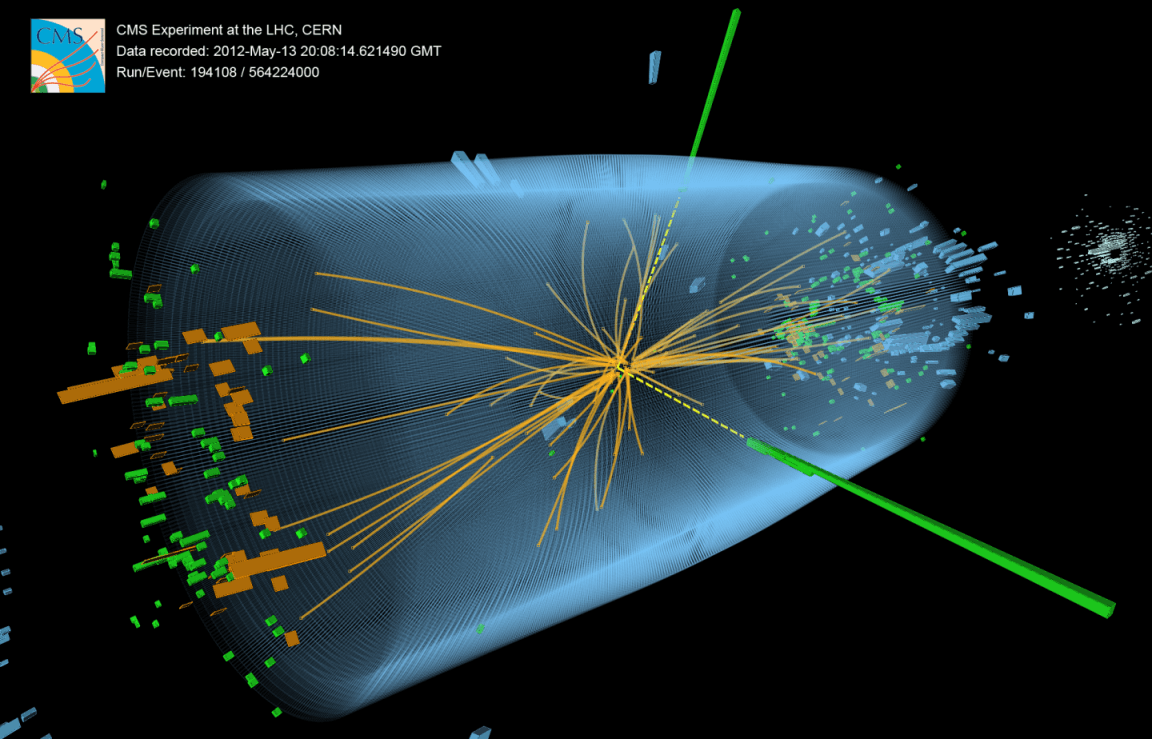
\includegraphics[scale=0.2]{Fotos/higgs-candidate.png}
					\end{figure}
					
				\end{minipage}}
				\onslide<2->{\begin{minipage}[c]{0.3\linewidth}
					\begin{figure}[t]
						\centering
						
\includegraphics[scale=0.3]{Fotos/masterclasses.png}
					\end{figure}
					
				\end{minipage}
				}

				\vspace{-1cm}

				\onslide<3->{\begin{minipage}[c]{1\linewidth}
					\begin{figure}[H]
						\centering
						
\includegraphics[scale=0.2]{Fotos/icecube.jpeg}
					\end{figure}
				\end{minipage}}

			\end{frame}

			\begin{frame}
				\frametitle{Muones y Dilataci\'on temporal}
				\onslide<1->{
				%\vspace{-0.2cm}
				\begin{minipage}[c]{0.3\linewidth}
					\begin{figure}[t]
						\centering
						
\includegraphics[scale=0.22]{Fotos/muons.png}
					\end{figure}
				\end{minipage}}
				\onslide<2->{\begin{minipage}[c]{0.6\linewidth}
					\begin{figure}[b]
						\centering
						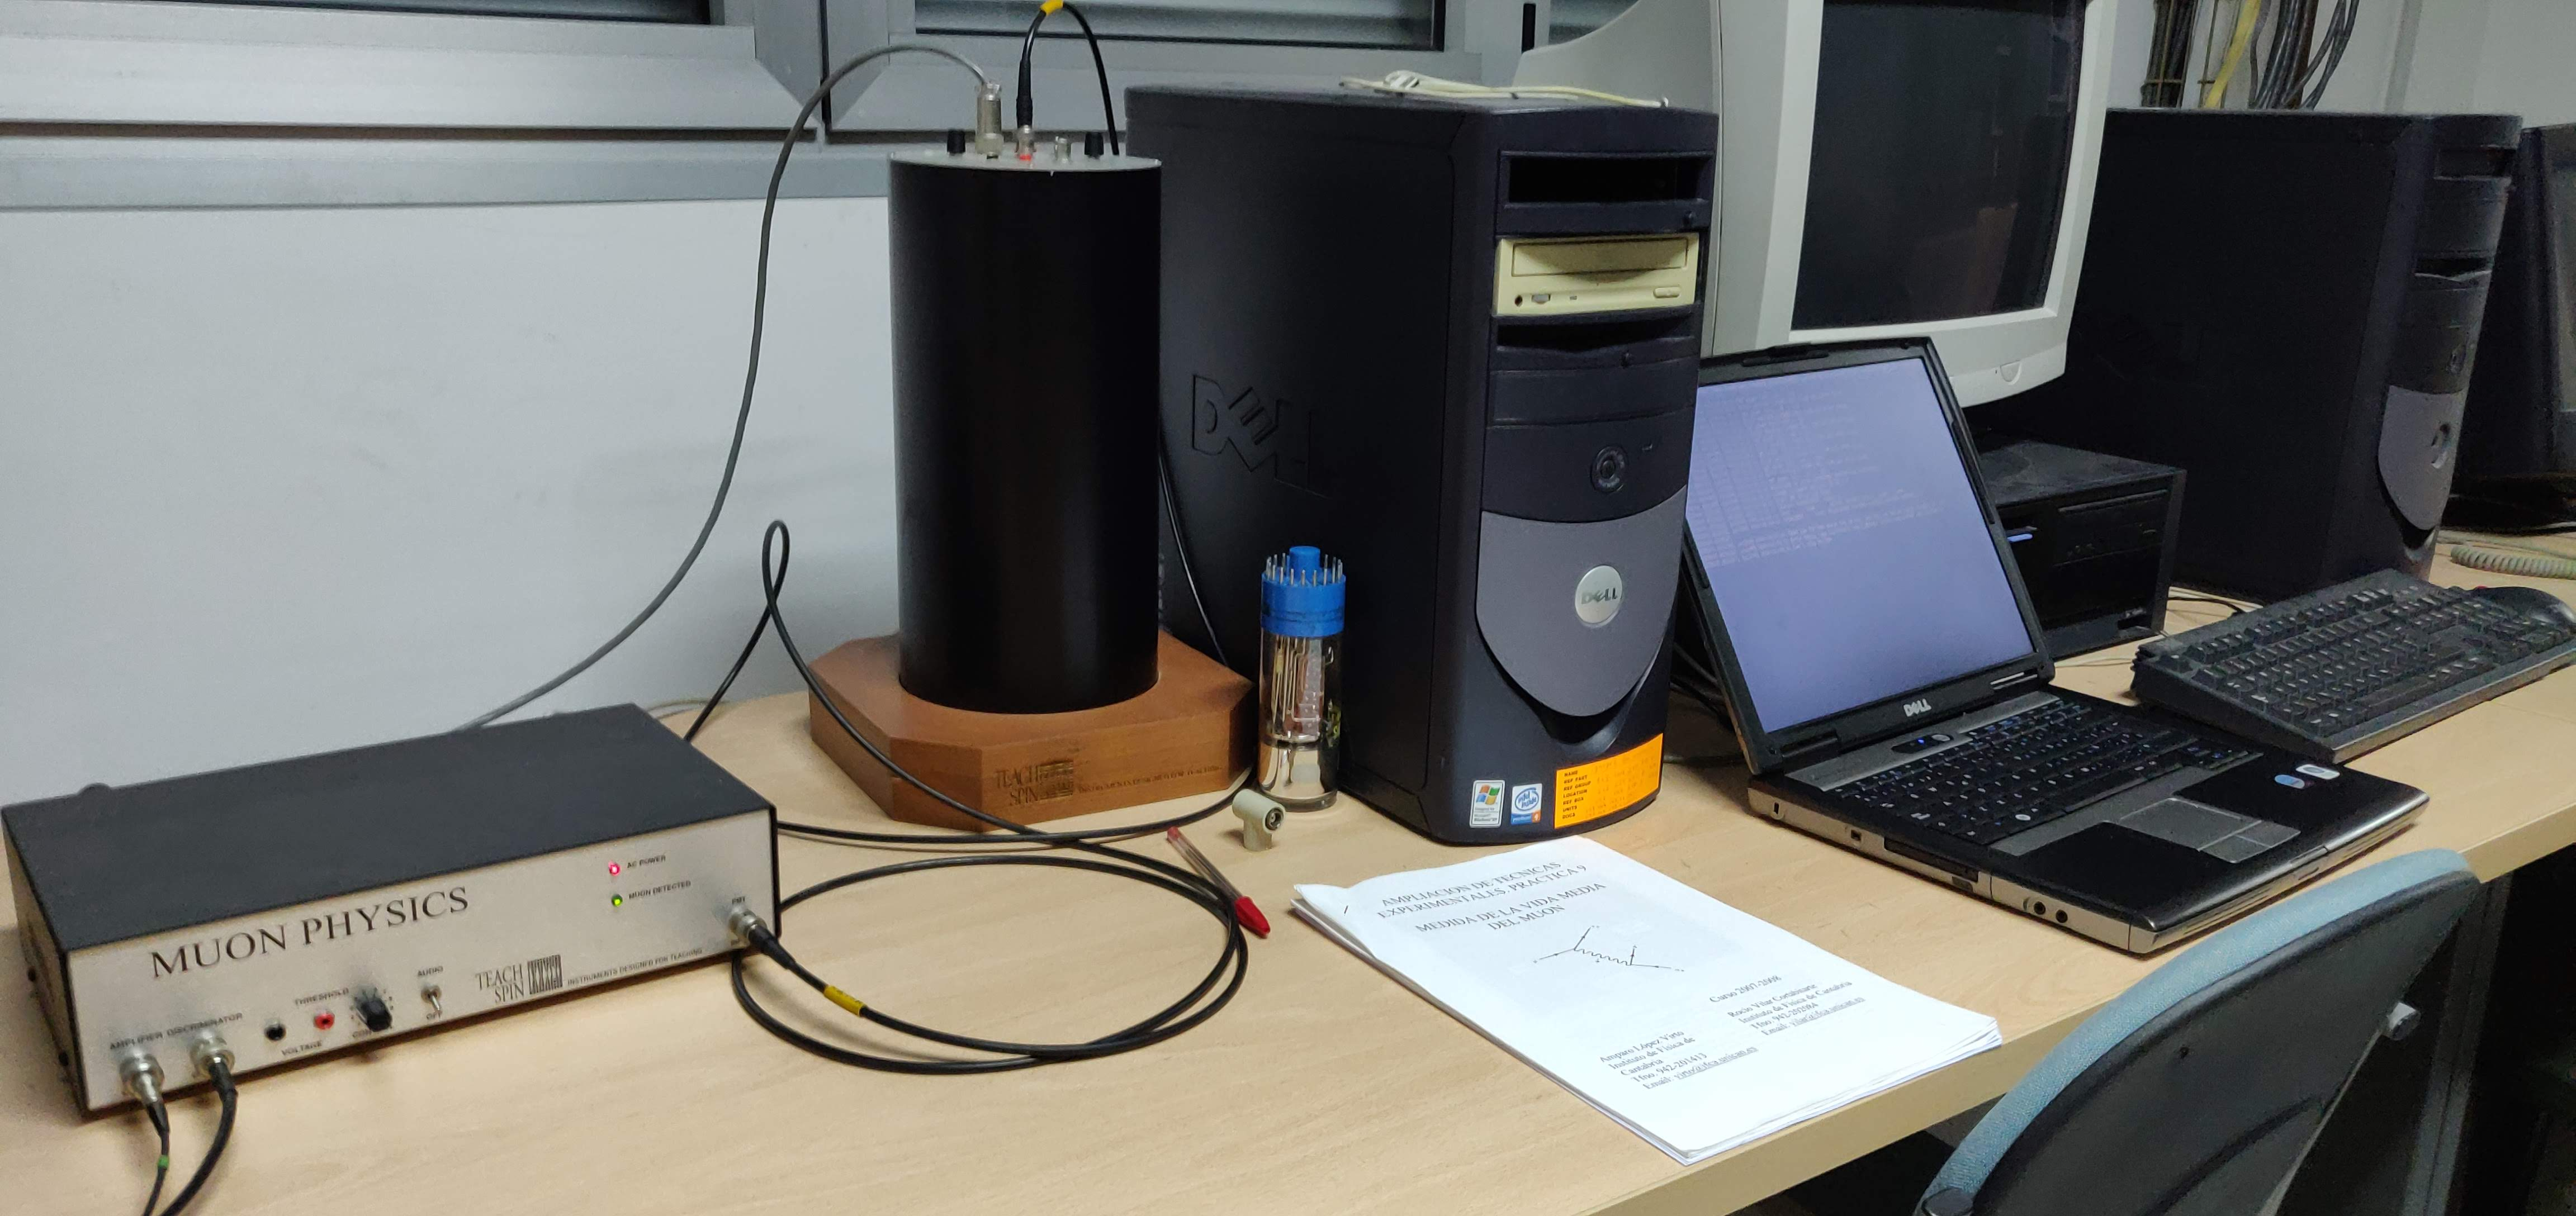
\includegraphics[scale=0.04]{Fotos/IMG_20180927_113646.jpg}
					\end{figure}
					
				\end{minipage}}
			\end{frame}

			\begin{frame}
				\frametitle{Red de Detecci\'on de Muones}
				\onslide<1->{
				\vspace{-3cm}
				\begin{minipage}[c]{0.3\linewidth}
					\begin{figure}[t]
						\centering
						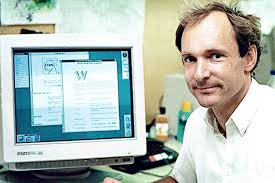
\includegraphics[scale=0.4]{Fotos/download.jpeg}
					\end{figure}
				\end{minipage}}
				\onslide<2->{\begin{minipage}[c]{0.6\linewidth}
					\vspace{3cm}
					\begin{figure}[b]
						\centering
						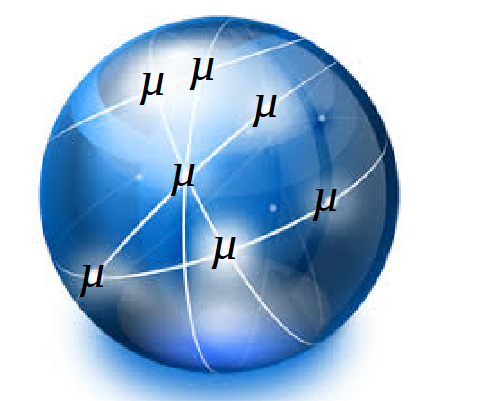
\includegraphics[scale=0.4]{Fotos/image.png}
					\end{figure}
				\end{minipage}}
				\onslide<3->{\begin{minipage}[c]{0.6\linewidth}
					\vspace{-1cm}
					{\fontsize{50}{60}\selectfont MuDeb}
				\end{minipage}}
			\end{frame}

			\begin{frame}
				\frametitle{2 dispositivos, 2 usos}
				\onslide<1->{
				%\vspace{2cm}
				\begin{minipage}[c]{0.3\linewidth}
					\begin{figure}[t]
						\centering
						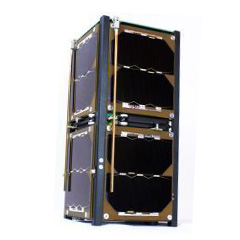
\includegraphics[scale=0.4]{Fotos/NanoRacks-ArduSat-2.jpg}
						%\caption{\footnote{Ejemplo del proyecto Infinity Aerospace’s ArduSat-2 \url{http://nanoracks.com/ardusat-demonstration/}}}
					\end{figure}
				\end{minipage}}
				\onslide<1->{\begin{minipage}[c]{0.6\linewidth}
					Autosuficiente gracias a sus paneles solares y con conectividad para poder acceder desde cualquier lugar del mundo a sus datos
				\end{minipage}}
				\onslide<2->{\begin{minipage}[c]{0.4\linewidth}
					\vspace{1cm}
					Más compacta y barata con varios puertos de conexión para la realización en un laboratorio
				\end{minipage}}
				\onslide<2->{\begin{minipage}[c]{0.5\linewidth}
					\vspace{1cm}
					\begin{figure}[b]
						\centering
						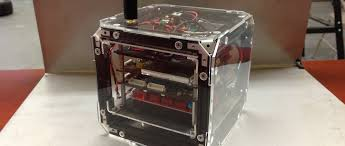
\includegraphics[scale=0.4]{Fotos/download(1).jpeg}
					\end{figure}
				\end{minipage}}
			\end{frame}


	%----------------------------------------------------------------------------
	%     BIBLIOGRAPHY
	%----------------------------------------------------------------------------

		\bibliographystyle{unsrt}
		\bibliography{biblio}

	\end{document} 